%%%%%%%%%%%%%%%%%%%%%%%%%%%%%%%%%%%%%%%%%%%%%%%%%%%%%%%%%%%%%%%%%%%%%%%%%%%%%%%%%%%%%
%																					%
%	TRABAJO: Paper Mejoras en el procesador de Redes de Petri						%
%																					%
%		Titulo: 	Soft Core parametrizable con procesamiento de Redes de Petri	%
%																					%
%		Autores:	Julian Nonino													%
%					Carlos Renzo Pisetta											%
%					Orlando Micolini												%
%																					%
%	Seccion: ANALSIS DE RENDIMIENTO													%	
%	Archivo: analisis_rendimiento.tex												%
%																					%
%%%%%%%%%%%%%%%%%%%%%%%%%%%%%%%%%%%%%%%%%%%%%%%%%%%%%%%%%%%%%%%%%%%%%%%%%%%%%%%%%%%%%

 \section{An�lisis de Rendimiento}
 		Una vez terminado el IP Core para comprobar su correcto funcionamiento y ver si �ste realmente 
 		tiene una mejora en los tiempos de sincronizaci�n, se realizaron mediciones para distinto n�mero
 		de iteraciones, tanto para el Procesador de Petro como para Sem�foros. La elecci�n de este segundo
 		m�todo de sincronizaci�n se basa en que son el mecanismo m�s ligero para realziar �stas tareas.
 		A partir de estas mediciones se realiz� la gr�fica de la Figura \ref{fig:resultados13} 
 		
		\begin{figure}[h]
			\centering
			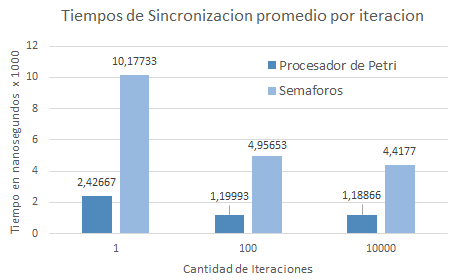
\includegraphics[width=3in]{./img/resultados13}
			\caption{Tiempos de sincronizaci�n procesador de Redes de Petri vs. Sem�foros}
			\label{fig:resultados13}
		\end{figure}		
		
		Se puede observar que, para todos los casos, el procesador de Petri es aproximadamente cuatro veces
		m�s rapido que los Sem�foros.
		Esta medicion se realizo con tiempos iniciales nulos, de manera que el rendimiento es el mismo obtenido
		en el procesador de Redes de Petri sin semantica temporal.
		\begin{figure}[h]
			\centering
			\includegraphics[width=3in]{./img/new01}
			\caption{Ejecucion transicion con tiempo}
			\label{fig:new01}
		\end{figure}	
		
		En la Figura \ref{fig:new01} se puede observar por que se analiza el rendimiento sin tener en cuenta
		el tiempo. Esto se debe a el tiempo EFT de una transicion es parte del modelo, es decir, el mismo que esperara la implementacion
		con semaforos; a la vez	el procesador necesita unicamente un semi-ciclo de reloj desde que el contador alcanza el valor hasta que se ve 
		representada a la salida y esta demora es despreciable en relaci�n con el tiempo que tiene un $\Delta$T de 
		un ciclo de reloj.
		
		
		 
		
		
		
		